\section*{Abstract}
    This paper explores the prospects of coherence prediction in distributed memory parallel machines, which has had little work since 2006. Motivated by the perceived opportunity nearly twenty years later, we rigorously examine the prospects of one form of coherence prediction: consumer prediction at the home site. Analyzing memory traces of the PARSEC 3.0 benchmark suite run on a parallel machine, we found that coherence prediction will not yield substantial benefits to performance due to a combination of a lack of shared cache line accesses, lack of many consumers for consumer prediction, and short history per shared cache line. Despite this finding, due to our limited workloads, we propose two consumer predictors: the LRU consumer predictor and the Override consumer predictor, at the home site. On two shared memory workloads, the LRU predictor achieves up to 89\% accuracy and the Override predictor achieves up to 94\% accuracy on all consumer predictions.

\section{Introduction}
    % To achieve better performance, computer architects have long turned to prediction mechanisms to hide latency-heavy events and remove dependencies between instructions. By predicting the future correctly, prediction mechanisms enable greater instruction level parallelism in a core as computation can continue without the need to wait on dependent instructions to finish. Such examples include branch prediction, which speculatively determines if a branch is taken or not taken using the history of that branch's behavior, cache replacement policies, which predict the re-usage interval of cache lines to maximize the effectiveness of the cache, and prefetchers, which issue fetches to higher level memories before it is needed by the processor to hide memory latencies. These prediction mechanisms are often specific to a single core, meaning that in a multi-processor system, these structures are duplicated per core. On typical consumer systems where users run many independent programs at the same time, this paradigm makes a lot of sense. When the programs are not independent, meaning that they share memory between processors, prediction mechanisms can suffer as they use information about what other processors are doing. \\

    In servers and data centers, shared memory parallel workloads are common. These particular systems are typically built from smaller processors that are strung together and use a shared memory paradigm since it is cheaper and more modular than a custom-built solution. This is known as a distributed shared memory (DSM) system. While many compute nodes and their main memories are physically connected together, the hardware hides much of the complexity, allowing the programmer to view the distributed main memory as one contiguous memory. The node that holds the main memory location of a memory address is known as the home site. As each system has its own memory hierarchy of caches and the address space is shared, directories are introduced as specialized hardware used to maintain coherence for each main memory. Each node's directory maintains information about which node in the system has access to its main memory as well as the state of each cache line of memory based on some coherency protocol. These directories arbitrate permissions between processors to make sure that memory is coherent between all processors. \\

    Assuming a MESI coherence protocol, for a processor to access an address whose main memory is not located locally to the processor, it must send a message over a common bus to the home site to request this information. This message would sit in a queue until the home site can process the request, and then reply. On the receiving end, the requester would have its own queue where it would not see that message until it is fully processed on its side as well. In the case that a node wanted to write and there were other nodes that previously shared the line, then the requester node would need to tell the home site to invalidate all other nodes' copies of the cache line so that it has the sole copy. At that point, the home site can then give the requester node access to write. This is illustrated in the worst case scenario number of network messages that need to be sent in figure \ref{fig:worst-case} for a three node DSM system. In this scenario, it is also possible that the home site processor has a copy as well, but this would not count toward the number of network messages as the shared processor is local to the home site and does not incur network costs. This figure also does not consider dropped messages or corrupted messages due to a lossy or busy networks. If there are multiple sharers, each of them need to acknowledge the invalidate from the home site. Depending on how busy they are, one write permission can take a long time to receive from the home site. Alternatively, if a shared line is going from one node that has write permission to a shared permission with many readers, the first read on the modified line will require the same amount of network requests as the previous scenario, but network request 2 goes to the node with modified access and is a request to go to shared. \\

    \begin{figure}[h!]
    \centering
    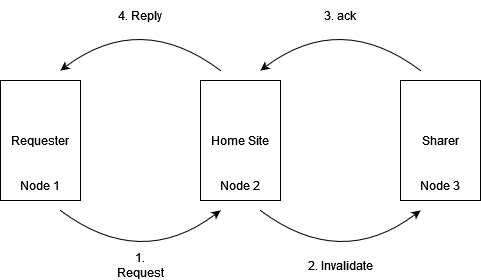
\includegraphics[scale=0.45]{img/worse_case.png}
    \caption{Worst Case Number of Messages in a 3 node DSM to maintain coherence}
    \label{fig:worst-case}
    \end{figure}

    To improve DSM performance, it is natural to consider whether it is possible to hide remote access latencies associated with maintaining coherence using prediction mechanisms. However, as there are many different coherency messages between nodes, one must determine Which coherence messages makes sense to predict to gain the most amount of performance. In figure \ref{fig:predictable-mesi}, we show a reduced MESI state diagram. It does not include processor transitions, as those can be represented by prefetchers. In addition, we do not include the inputs that do not cause state transitions. At this point, the state transitions can be broken up into three categories: invalidation prediction, consumer prediction, and shared permission prediction. Invalidation prediction is shown in purple and means that at the processor side, can we speculatively predict that a line will get invalidated and invalidate a line before it is explicitly asked by the home site. Orange shows reader, or consumer prediction. If we are in a modified state, can the home site predict who in the future will be a reader. Lastly, we show shared permission prediction in green, which is similar to invalidation prediction, in which we try to predict a reactionary message from the homesite speculatively. We focus specifically on consumer prediction in this study. 

    \begin{figure}
        \centering
        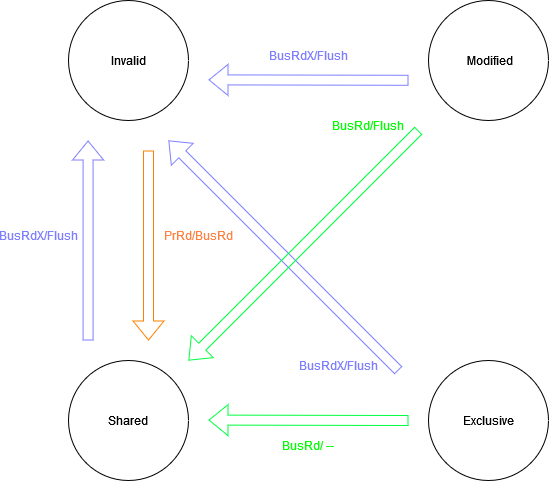
\includegraphics[scale=0.3]{img/reduced_interesting_mesi.drawio.png}
        \caption{Reduced MESI protocol for interesting coherence. Purple is invalidation prediction, orange is consumer prediction, and green is shared permission prediction}
        \label{fig:predictable-mesi}
    \end{figure}

\subsection{Contributions of this Paper}
    In this paper, we analyze the shared memory access patterns and their frequencies in the PARSEC 3.0 \cite{zhan_parsec3.0_2016} benchmark suite, a conglomeration of modern, shared memory, parallel workloads to determine the possible performance improvements of invalidation prediction and consumer prediction. We then propose two consumer predictors: the LRU consumer predictor and the Override consumer predictor, which are two-level table-based predictors that would sit at a homesite and speculatively identify readers after a write request.

\section{Related Work}
    The first paper that attempts coherence prediction is the Mukherjee and Hill paper in 1998, who proposed the Cosmos predictor, an adaptation of Yeh and Patt's two level branch predictor \cite{yeh_two_1991} to predict the next coherence message at the directory and at each processor's cache. Previous work on coherence prediction focused on profiling benchmarks before runtime or using compiler hints to tell the processor what to do, but this solution could adapt to any benchmark with no prior knowledge. On five separate scientific applications (\textit{Appbt, Barnes, Dsmc, Moldyn, and Unstructured}), the Cosmos predictor resulted in next coherence message prediction accuracy ranging from 69\% to 93\%. This study was done outside of a simulator, such that there was no speedup information, but this paper proved that predicting coherence messages may be a worthwhile avenue to pursue for parallel machines with long network latencies. \\

    Shortly after, Lai and Falsafi in 1999 build off the work from the previous year with their memory sharing predictor (MSP) \cite{lai_memory_1999}. Rather than predict all possible coherence messages, they only predict request messages such as permissions to write and read. They implement a speculative write invalidation, which determines when a processor is done writing and invalidates itself to forward information back to the homesite. When predicting consumers in a producer-consumer scheme, they make the problem more simple by simply predicting which processors will use a line without worrying about order.They achieve better prediction accuracy than the Cosmos predictor with less memory overhead due to not storing or predicting acknowledgments. \\

    In that same year, Kaxiras and Young presented a taxonomy of prediction schemes on predicting consumers in a producer-consumer scheme \cite{kaxiras_coherence_1999}. They found that the consumer prediction is where most of the speedup for coherence prediction will come from. They found that the processor ID and the depth of history stored have the most impact on coherence prediction. The memory address also matters, but the instruction program counter matters much less. Finally, this work analyzes the impact of coherence prediction schemes as a tradeoff between latency and bandwidth. With more messages and more predictions being sent onto the network, the average latency should drop given good accuracy, but the amount of messages will increase the amount of network traffic on shared buses, where we may lose performance due to network congestion. Therefore, they state that it is necessary to consider reasonable coherence predictors that limit the amount of traffic that they generate on the network, similar to the argument against very deep prefetchers. \\

    In 2006, Leventhal and Franklin picked up coherence prediction, but focused on consumer predictor using another augmented branch predictor, the perceptron \cite{leventhal_perceptron_2006}. By using a perceptrons, they decoupled the total history storage from the predictor, allowing for history length to scale linearly in memory space rather than exponentially in previous two-table schemes. They show that a processor's own history is the greatest indication of whether it will be a sharer of a line in the future, but more interestingly, they show that the information about whether other processors were also consumers, can impact whether that particular processor will be a sharer in the future. Using perceptrons to weigh the relative importance of different processor memory traces, they predict consumers with a global history. \\

    While our work is similar, we run on a modern benchmark suite to determine whether the additional hardware is worth it for consumer prediction and propose novel approaches toward consumer prediction. 

\section{Consumer Prediction}
    To tackle the consumer prediction problem, we modify the Cosmos two-level predictor \cite{mukherjee_using_nodate} to predict which processors will be a consumer of a particular write rather than general coherence messages. Like Cosmos, we keep track of the processor ID, as well, but only home site requests (reads and writes) rather than all messages. Cache line access patterns between processors may be similar throughout the history of a workload, allowing to predict who may be the next readers after a write occurs. In the next sections, we discuss our baseline model, a modification of the Cosmos predictor, and then a secondary implementation that further improves performance by modifying the pattern history replacement policy of our first implementation.
    
    \subsection{LRU Predictor}
    Similarly to the Cosmos predictor, our consumer predictor requires, both a Message History Table (MHT) that consists of Message History Registers (MHR) and Page History Tables (PHT). Each cache line in the homesite is assigned a MHR in the MHT, that tracks a series of the tuples of (proc\_id,(Read/Write)), which correspond to the last few memory operations the home site received for that cache line. We refer to length of the last tuples as the depth of the MHR. Each cache line has its own PHT that is indexed by the series of tuples that are saved in the MHT.\\

    We modify Cosmos' PHT, which would predict a coherence protocol message, to predict a one-hot bit array, where each bit represents whether a processor will be a consumer or not. One issue arises though in that we need to be able to update a particular entry in the PHT long after the MHR for that cache line has been updated by various reads. To do so, we introduce an additional table, the PHT Index Table (PIT), where each cache line is assigned an entry and tracks what the MHR was at the time of the last write to that cache line, essentially, what index in the PHT should be upgraded. Every time the home site receives a read request, it updates the cache line's PHT using its entry in the PIT and the processor id. A prediction is then made on every RWITM, simply by indexing into the PHT using the cache line's current MHR.\\    
    
    Each PHT is constrained to some limited size, thus in our initial solution, the replacement policy for lines in the PHT was simply LRU. However, this poses a problem. Since the bit array values are only upgraded to consumer and never downgraded, the only way to fix changed pattern behavior or ruined entries is through LRU. The next implementation addresses this issue.

    \subsection{Override Predictor}
    To address the issue of overstaying faulty consumer predictions, we introduce a final table, the Consumer History Table (CHT), which tracks which processors have requested the latest write to the cache line. This table is updated after each read request that the home site receives in place of updating the PHT. Then, after each RWITM for a cache line the cache lines at the PIT entry in the PHT is overridden with the CHT for that cache line. While we still rely on LRU to kick out entries in the PHT when it full, we no longer rely on it to downgrade predictions to non-consumers.

\section{Methodology}

    \subsection{Test Setup}
        All memory trace runs were performed on the Texas Advanced Computing Center (TACC)'s Lonestar6 cluster. Each compute node on a cluster consists of two AMD EPYC 7763 64 core processors. Each node has 256 gigabytes of DDR4 main memory. In our tests, we run with one node with 32 cores dedicated to running the benchmark. \\

        To gather memory traces of the system, we used Intel's 3.2.8 PIN binary instrumentation tool with a custom written PIN tool. This PIN tool captures all memory accesses per process as well as lock acquisitions and failed locks per process to mark race conditions for shared memory locations under contention. To make memory trace acquisition quicker, we only capture memory trace information after the second process has started performing memory accesses. Almost always in parallel benchmarks, the setup is done with one process and the actual benchmark does not begin until multiple processes are actively working in parallel. Since we are concerned with shared memory contention, we start collecting memory trace information then.

    \subsection{Benchmarks}
        We use PARSEC 3.0 \cite{zhan_parsec3.0_2016}, a collection of shared-memory parallel programs, to gather memory traces from. Out of the 10 available benchmarks, we use 7 benchmarks, excluding ferret, facesim and x264 due to input compilation errors. All benchmarks were run on the small input and are run for 30 minutes or until completion on the TACC Lonestar6 machine. For the benchmarks available all of them are data parallel: blacksholes is a financial analysis tool, bodytrack is a computer vision workload, facesim is an animation benchmark, fluidanimate is a fluid animation simulation, freqmine is a data mining application, raytrace is a highly independent rendering workload, swaptions is a parallel economics application, and vips is a media processing tool.

    \subsection{Speculative Invalidation Setup}
        To develop an invalidation prediction scheme, an oracle is first needed to test our invalidation prediction scheme against. Using our global memory traces, we create an oracle as follows: if processor A is writing to a shared memory address, all other processors invalidate that local cache line copy. Each benchmark memory trace is parsed, with invalidates for each processor being placed directly before the write of a processor. With these remote invalidations in hand, we recreate each processor's memory trace, with remote invalidations added. Without explicit timing of when invalidates would arrive to remote processors, it is impossible to recreate the processor's trace to get an accurate oracle to what happened at runtime. For this reason, we did not continue.

    \subsection{Accuracy Metrics}
        When calculating whether or not a consumer prediction is accurate or not, we use a pessimistic definition of accuracy, requiring that every single prediction per processor is accurate since incorrect predictions are expensive. For example, if we have 32 processors, on a consumer prediction query, for it to be correct, we must predict whether every single processor will use or not use that written line. If it is off by a single processor, we mark the prediction as incorrect.

\section{Experimental Results}
    \subsection{Statistical Analysis of Benchmark Memory Traces}
                \begin{table}[h!]
        \centering
        \resizebox{\textwidth}{!}{%
        \begin{tblr}{|p{1in}|p{0.8in}|p{0.8in}|p{0.8in}|p{1in}|p{1in}|p{1in}|p{1in}|p{1in}|p{1in}|}
        \hline
        \textbf{Benchmark}    & \textbf{Shared Cache Lines \% (Total)} & \textbf{Shared Cache Lines \% (Program)} & \textbf{Shared Cache Line \% (OS)} & \textbf{Average Unique Consumers per Prediction (Total)} & \textbf{Average Unique Consumers per Prediction (Program)} & \textbf{Average Unique Consumers per Prediction (OS)} & \textbf{Average Predictions per Shared Cache Line (Total)} & \textbf{Average Predictions per Shared Cache Line (Program)} & \textbf{Average Predictions per Shared Cache Line (OS)} \\ \hline
        blacksholes  & 0.06\%                                 & 0\%                                      & 100\%                              & 32                                                       & 0                                                          & 32                                                    & 1                                                      & 0                                                        & 1                                                   \\ \hline
        \textbf{bodytrack}    & \textbf{12.37\%}                       & \textbf{0.65\%}                          & \textbf{99.35\%}                   & \textbf{1.66828271}                                      & \textbf{2.991071429}                                       & \textbf{1.480522946}                                  & \textbf{6.962179748}                                   & \textbf{133}                                             & \textbf{6.136717151}                                \\ \hline
        facesim     & 0.24\%                                 & 0.00\%                                   & 100.00\%                           & 2.208955224                                              & 0                                                          & 2.208955224                                           & 22.33333333                                            & 0                                                        & 22.33333333                                         \\ \hline
        \textbf{fluidanimate} & \textbf{11.14\%}                       & \textbf{95.55\%}                         & \textbf{4.45\%}                    & \textbf{1.198496122}                                     & \textbf{1.101855807}                                       & \textbf{1.668513389}                                  & \textbf{1.631301779}                                   & \textbf{1.416117758}                                     & \textbf{6.251082251}                                \\ \hline
        freqmine     & 0.47\%                     & 98.55\%                                  & 1.45\%                             & 2.259865255                                              & 1.908146528                                                & 4.843373494                                           & 1.366655705                                            & 1.220553887                                              & 11.31818182                                         \\ \hline
        raytrace              & 4.71\%                                 & 0                                        & 100.00\%                           & 1.84496124                                               & 0                                                          & 1.84496124                                            & 4.3                                                    & 0                                                        & 4.3                                                 \\ \hline
        swaptions             & 0.24\%                                 & 100.00\%                                 & 0.00\%                             & 3.649038462                                              & 3.649038462                                                & 0                                                     & 9.043478261                                            & 9.043478261                                              & 0                                                   \\ \hline
        vips                  & 0.03\%                                 & 0                                        & 100.00\%                           & 3.765625                                                 & 0                                                          & 3.765625                                              & 2.37037037                                             & 0                                                        & 2.37037037                                          \\ \hline
        \end{tblr}%
        }
        \caption{Statistics on PARSEC benchmarks detailing the percentage of cache lines, number of unique consumers per producer, and number of possible queries per shared cache line (with cache line size of 128 bytes). Each statistic is further split into OS calls (os space addresses) and Program calls (user space addresses)}
        \label{tab:statistics}
        \end{table}
    
        After obtaining memory traces from TACC, we analyzed the traces to obtain relevant statistics for each PARSEC benchmark to determine the headroom possible from coherence prediction. This information is reported in Table \ref{tab:statistics} with a cache block size of 128 bytes. The table shows three unique statistics, and for each, splits them into OS space addresses and user space addresses. While both can be predicted on, this separation explicitly shows OS dependence on acquiring and arbitrating locks and other operating system callbacks that require memory accesses. The three unique statistics are the percentage of shared cache lines, the average number of consumers per possible prediction, and the average number of predictions per shared cache line. A prediction is triggered by a write or producer, and predicts which processors will read this line. All three of these statistics together paint a picture of the possible opportunity for coherence prediction as this mechanism can only predict on shared cache lines. The more unique consumers per possible prediction (a write arrived and we need to predict the readers), the more latency we can hide on updated information. This statistic also gives us the average amount of readers that could be invalidated before another producer needs to write for invalidation prediction. The last statistic on average predictions gives us an estimate on how we might need to train a system. If there is a limited number of predictions per cache line, it means the prediction strategy needs to be somewhat abstracted from the cache line. \\
    
        Starting from left to right, the benchmarks with the greatest percentage of shared lines are \textit{bodytrack} and \textit{fluidanimate} at 12.37\% and 11.14 \%, respectively. These two benchmarks are bolded in the table. While \textit{raytrace} also has a large percentage of shared lines 4.71\%, its runtime is very short and there are not many memory accesses, leading to a higher percentage of shared lines even though they originate only as OS locks. The rest of the benchmarks: \textit{blacksholes}, \textit{facesim}, \textit{freqmine}, \textit{swaptions}, and \textit{vips} have little to no sharing since they the data they work on is fairly independent. \\
    
        Of the two highlighted benchmarks, \textit{bodytrack} shared cache line accesses are primarily coming from the operating system address space, while \textit{fluidanimate} primarily comes from the user address space. The average amount of unique consumers per prediction at 1.66 and 1.19, respectively, suggest that most of the time, after a shared cache line write, it is only read by one or two other processors, on average. This does not bode well for consumer prediction or speculative invalidation in coherence prediction, as both achieve more performance gains by removing possible dependencies when there are many consumers. The last statistic shows that for both benchmarks, the OS space addresses seem to be reused somewhat regularly, which would most likely be arbitrating access to a lock. The last interesting thing in \textit{bodytrack} is that the program user address, \textit{bodytrack} seems to have a small cache area of shared memory that is used fairly regularly in a somewhat regular producer-consumer scheme. \\
        
        Overall, this statistic demonstrates that the average number of predictions per shared cache line is still fairly low for these benchmarks, suggesting that an effective solution would need to try and hash the cache line address to get more history to train on. In addition, for both invalidation prediction and consumer prediction, the statistics seem to suggest that there are very limited performance improvements, even with perfect predictors.

    \subsection{Consumer Prediction Result}
        To test our consumer prediction schemes, we consider the \textit{bodytrack} and \textit{fluidanimate} benchmarks as our statistical analysis showed that these benchmarks had the greatest opportunity for consumer prediction. Based on the MHR depth recommendation of the Cosmos predictor, we use a depth of 3 \cite{mukherjee_using_nodate}. In figure \ref{fig:initial-results}, the override consumer predictor achieves greater accuracy on both benchmarks over the LRU predictor. While not shown in the figure, we performed runs on the \textit{blacksholes} benchmark which achieved 0\% accuracy due to a lack of repetitive shared line history.  

        \begin{figure} [h!]
            \centering
            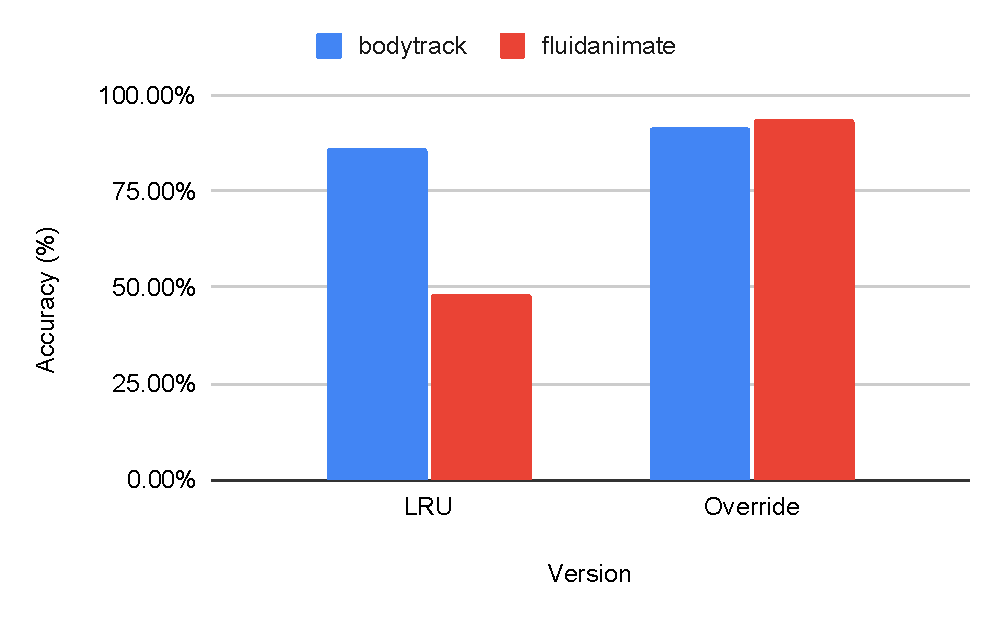
\includegraphics[scale=0.5]{img/initial.pdf}
            \caption{Prediction accuracy with 1-bit per processor in the PHT entry and an MHR history depth of 3. }
            \label{fig:initial-results}
        \end{figure}

        \subsubsection{Bit Sensitivity}
            We also examine the bit sensitivity of the PHT per processor. In figure \ref{fig:bit-sensitivity}, we run the LRU predictor and Override predictor with 1 bit per processor, and 2 bits per processor as a saturating counter. Since each processor in the bit array would require an additional bit in the 2-bit saturating scheme, adding an additional bit would double the memory size of the PHT. On \textit{bodytrack}, increasing the number of bits per processor very slightly increases accuracy of the predictors, but not in a significant manner. The same trend is observed in \textit{fluidanimate}. In future runs, we use one bit per processor for the PHT as the benefit to accuracy does not outweigh the additional memory overhead. 
        
    
            \begin{figure}[h!]
                \centering
                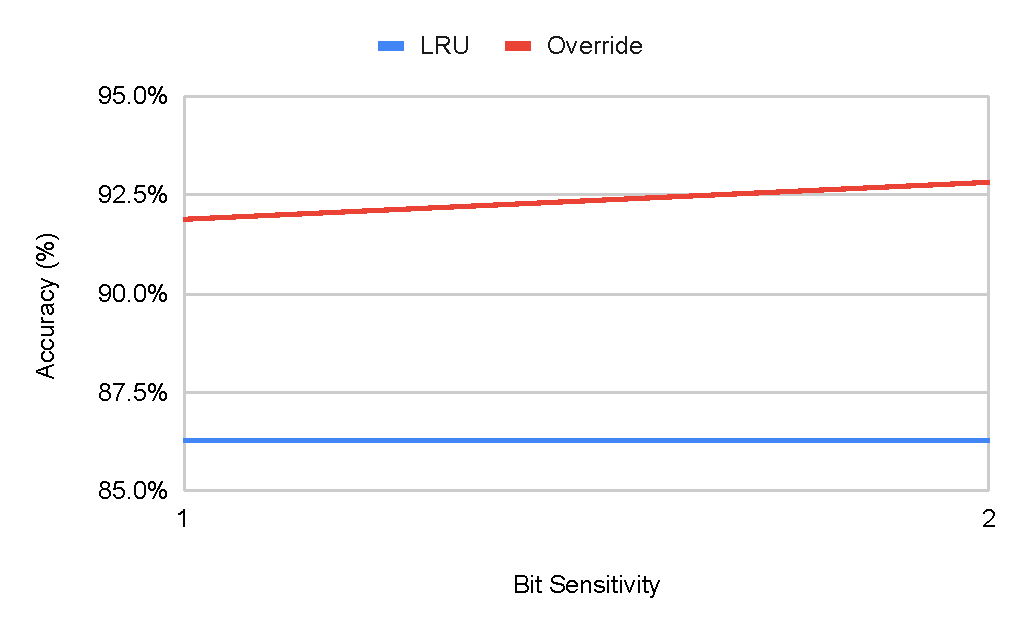
\includegraphics[scale=0.5]{img/bit_sensitivity.pdf}
                \caption{Bit sensitivity per processor in a PHT entry on \textit{bodytrack}.}
                \label{fig:bit-sensitivity}
            \end{figure}

        \subsubsection{MHR Depth Sensitivity}
            We examine the MHR depth sensitivity of our two prediction schemes in figure \ref{fig:depth-sensitivity} and find that the override predictor still performs well with less MHR history, but that is not the case for the LRU predictor. We believe that the LRU predictor is more sensitive, as it gets rid of PHT entries based on the PHT being full. Since the MHR history hashes into the PHT, a smaller history creates aliasing which negatively affects performance. With the greatest depth possible, the LRU predictor achieves a maximum accuracy of 89\% on bodytrack and the Override predictor consistently achieves 92\% irrespective of history depth.
    
            \begin{figure}[h!]
                \centering
                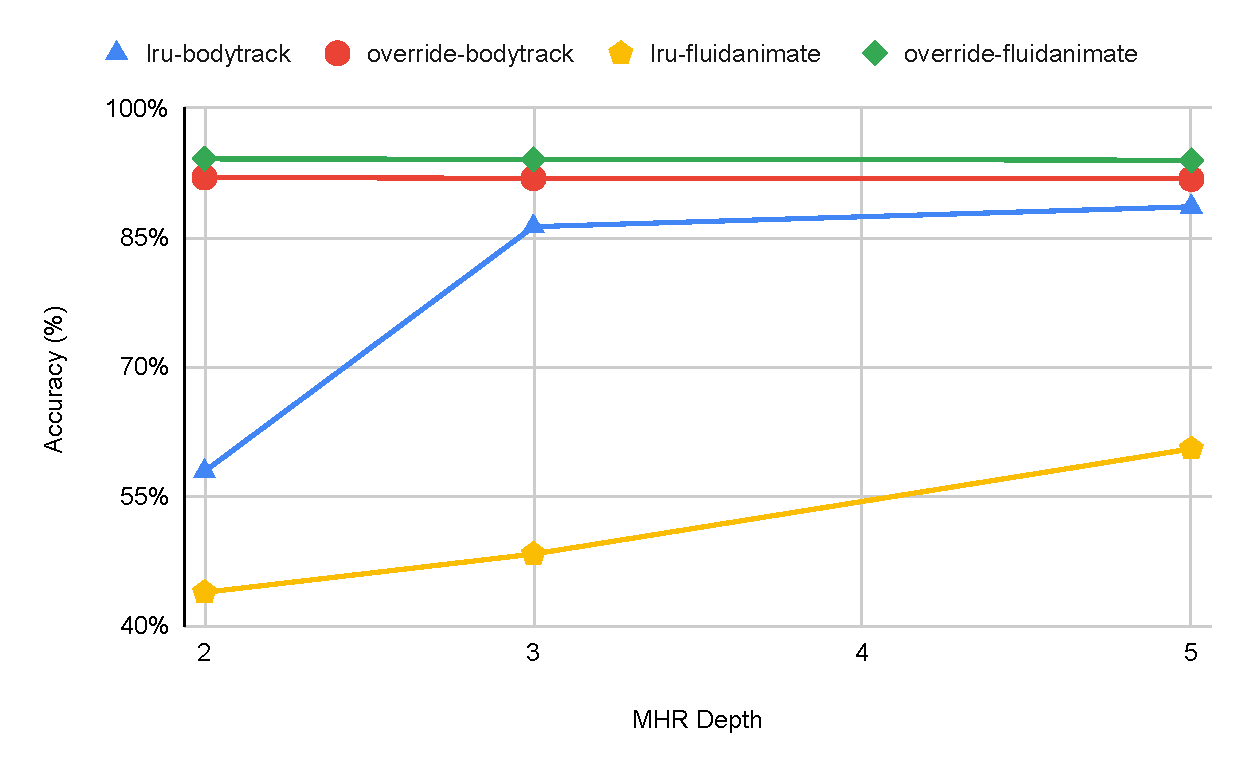
\includegraphics[scale=0.45]{img/history_depth_sensitivity.pdf}
                \caption{MHR depth sensitivity on consumer prediction accuracy with one bit per processor in the PHT.}
                \label{fig:depth-sensitivity}
            \end{figure}


\section{Conclusion}
    Revisiting the landscape of coherence prediction for distributed memory parallel machines, our study performs a statistical analysis of parallel memory traces from the PARSEC 3.0 benchmark suite. As anticipated, the current software paradigm for parallel programs dictates that shared memory between processors should be limited to a minimum as any synchronization reduces performance. Our statistical analysis confirms this paradigm for PARSEC, as only a small subset of workloads have many shared lines. Of those shared lines, there is a limited number of consumers per producer, and little history to train on, limiting the performance improvements of consumer prediction while making the prediction problem difficult. \\

    We develop two, two-level table-based consumer predictors: the LRU consumer predictor and the Override consumer predictor. The LRU consumer predictor achieves 44\% to 89\% accuracy on consumer prediction at the home site while the Override consumer predictor is able to achieve 91\% accuracy to 94\% accuracy. We explore the PHT bit sensitivity per processor as well as the history depth required for these table-based solutions and found that the Override predictor performs well, even with the least amount of history and bits per processor tested. On shared-memory parallel workloads that share more memory than those tested in our study, these consumer predictors may make sense as an additional avenue to hide remote access latencies.
    
\section{Future Work}
    To better confirm our findings, we plan to fix the three benchmarks (\textit{ferret}, \textit{x264}, and \textit{facesim}) for the PARSEC 3.0 benchmark suite. In addition, we plan to run all benchmarks on a larger number of cores as well as run the full benchmark on a larger input set. Since the PARSEC benchmark does not include all types of modern workloads, particularly in the data centers which may have more explicit consumer-producer schemes, we plan to investigate a larger swath of modern workloads using our methodology to further confirm our findings. Furthermore, we plan to to implement the consumer predictors proposed in a cycle-accurate simulator to evaluate possible speedup. We plan to explore PHT sensitivity for our coherence predictors as well as the total memory footprint. Relating to home site message prediction (invalidation prediction and shared permission prediction), after creating the oracle, it still remains a question whether branch prediction methods can be applied. 

\section{Division of Labor}
    \begin{enumerate}
        \item \textbf{Preston Glenn:} Developed scripts to clean memory traces. Designed and the various Consumer Predictor architectures. Implemented the predictors as Python. Ran all jobs related to consumer prediction.

        \item \textbf{Jason Ho:} Developed PIN tool to gather memory traces from PARSEC benchmarks while annotating lock acquisition, and lock failures due to shared memory contention. Performed statistical analysis on benchmark traces to generate table 1 and analyssis of raw data from consumer prediction runs. Wrote abstract, introduction, related work, methodology, statistical analysis of benchmark memory traces for report, consumer prediction results section, and the conclusion. Created presentation slides as well.
     

        \item \textbf{Madison Threadgill:} Set up, fixed, and managed PARSEC benchmark suite on TACC along with gathering relevant input traces. Managed and monitored runs for all memory traces. Attempted (for long hours) to develop an invalidation prediction oracle. Wrote the invalidation prediction part of the report.
    \end{enumerate}

\section{Trials and Tribulations}
    PARSEC and PIN were very difficult to install as the Parsec website is no longer active, however, we were able to get the data from other students. Obtaining the oracle for the invalidation prediction scheme was difficult as our sequential memory trace does not make it clear when an invalidate will arrive at a processor to invalidate the line as PIN does not explicitly provide ways to access to coherency trace.
    
